\chapter{Introduction \todol{todo}}

%\mycomment{OR: Finde diese ``remarkable similarities'' etwas zu stark betont.
%Wenn man die ganze Bandbreite an Anwendungen anschaut sind sie in Wahrheit nicht gross.}
High-performance sparse solver libraries have 
played an important role in
scientific and engineering computing for years. Their importance still
continues to grow as microprocessor architectures become more complex
and as, at the same time,
software libraries become better designed to integrate easily
with
applications. 
%
Despite %\sout{the fact}
the large variety of
science and engineering applications, the underlying algorithms typically have
remarkable similarities, especially those algorithms that are most
challenging to implement well in parallel. 
It is not too strong a
statement to say that %\sout{these} 
sparse solver
%\mycomment{OR: ``these'' hat keinen Bezug. MW: OK.
%OR: ``these'' hat immernoch keinen Bezug. Es ist davor von ``algorithms with
%remarkable similarities'' die Rede. Die ``sparse solver libraries'' werden auf
%der Seite davor erwaehnt. MW: OK
%}
%\sout{software} 
libraries are essential to the
broad success of scalable high-performance computing in computational
sciences. 

The recent trends in hardware development have added
additional 
uncertainty
to this scenario 
because today's codes are not
guaranteed to exploit the performance of next-generation hardware 
well.
The so-called memory wall, i.\,e., the increasing
performance gap between memory bandwidth and processor speed, will force
scientific computing software to %\sout{deal with }
%\sout{the efficient use of}
%\sout{the efficient} {\MW efficiently} 
use %\sout{of}
%\mycomment{MW: ``the efficient use of'' wuerde ich lassen, weil benutzen kann man komplexe Speicherhierarchien auch ineffizient; OR: ``deal with the efficient use'' heisst auch nicht, dass man es effizient macht. MW: besser ``efficiently use complex...'' OR: So finde ich es gut.}
complex multiple memory hierarchies.  

%%- \begin{figure}[t]
%%-     \centering
%%-   \subfloat[forward subst.]{
%%-         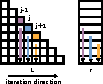
\includegraphics[width=0.35\linewidth,clip=true]{images/forward-small}
%%-   } \, \hspace{0.5cm}
%%-   \subfloat[backward subst.]{
%%-         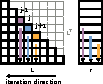
\includegraphics[width=0.35\linewidth,clip=true]{images/backward-small}
%%-   }
%%-   \caption{Sparse triangular substitution in compressed sparse column format.}
%%-   \label{algo:triangular}
%%- \end{figure}


In this work, we will focus on 
sparse
%\mycomment{OR: Ohne ``sparse'' braeuchten wir kein Pardiso. MW: OK}
systems of linear equations that arise
at the heart of many scientific and engineering applications. 
Many of these linear systems are sparse, i.\,e., most of the 
% \mycomment{OR: ``element'' sollte in unserem Kontext besser fuer ``finite
% element'' reserviert bleiben. MW: OK}
entries 
in the
coefficient matrix are zero. 

%mw20810607: \mycomment{OR: Hier lieber was mit Bezug zum Projekt. MW: das muesste jemand
%mw20810607: anderes scheiben, mir fehlt dazu der Ueberblick.
%mw20810607: OR: OK. Ich versuche es bei Gelegenheit.
%mw20810607: }
%mw20180607: \uwave{
Direct methods based on matrix
factorizations are sometimes needed to ensure accurate solutions. For
example, accurate solution of sparse linear systems is needed in
shift-invert Lanczos to compute interior eigenvalues. The performance
and resource usage of sparse matrix factorizations are critical to
time-to-solution and maximum problem size solvable on a given
platform.
%mw20180607: }

In many applications, the coefficient matrices are
symmetric, and exploiting symmetry will reduce both the amount of work
and storage cost required for factorization. We consider direct
methods for solving a sparse symmetric linear
system, which are based on Cholesky or $LDL^T$
factorization. While direct
methods can be expensive for large matrices, in terms of execution
times and storage requirement when compared to iterative methods, they
are quite robust also for ill-conditioned systems 
where standard preconditioned Krylov methods struggle with convergence.
Indeed, iterative methods of the domain decomposition family often apply
direct sparse solvers as building blocks to achieve robustness, e.\,g., with respect 
to ill-conditioning from large heterogeneities inside subdomains or almost incompressibility.
%\sout{have the advantage that they terminate in a finite number of
%operations.} 
%mw2018-06-07: \mycomment{OR: ``finite number of ops''!?}
%mw2018-06-07: \mycomment{TODO OLAF: OR: Lieber auf unseren DD-Kontext umformulieren. Wir sollten hier keinen Dualismus iterativ/direkt aufmachen. Lieber die Synergie betonen.}
%\sout{Also, direct methods can handle linear systems that are
%ill conditioned or the situation when there are many multiple
%right-hand sides.}


We are, in particular, interested in the forward and backward solution
process of sparse direct solvers since they build 
a
computational
kernel, e.g., of domain decomposition solvers~\cite{toselli:2005:ddm}
with exact (i.e., direct sparse) local and/or coarse solvers. 
We will thus consider the forward/backward subst.\ phase
of the PARDISO~\cite{schenk-2004} sparse direct solver which
is used in our nonlinear FETI-DP domain decomposition
solver~\cite{klawonn:2015:tes} applied in our project EXASTEEL for the
simulation of dual-phase steels.
% ~\cite{klawonn2002dual}. 
Implicit finite element solvers of the FETI-DP or BDDC type are known to be highly
parallelizable and can use as building blocks efficient preconditioners
or, preferable for high robustness, direct sparse solvers.


We will investigate and analyze
the performance of the forward/backward solution process of 
the
PARDISO %~\cite{schenk-2004} 
direct sparse solver
and present not only numerical
results, but also a detailed performance analysis for its sparse solver kernel.
This analysis is based on the Roofline model~\cite{williams-2009}, a resource-driven and
practically applicable model, and describe the performance of sparse
kernel loops~\cite{Gropp99,Williams:EECS-2008-164,KHWPAF14}.
%
We establish a modified Roofline model that captures the serial and parallel
execution phases which allows us to predict the in-socket scaling over the
processor cores.
This distinction is important as the amount of the serial fraction depends on
the matrix used and can have a significant negative impact on performance.

The performance analysis and modeling performed in this paper is limited to a
single node, however, the code considered here is also a building block for the
MPI parallel version. 
%mw2018-06-07: \mycomment{TODO OLAF: MW: Olaf, hast du dazu noch eine Referenz?}
Hence, also the distributed memory implementation will profit from any
enhancement achieved.

% the performance of the forward/backward solution process of libraries
% such as CHOLMOD~\cite{doi:10.1137/1.9780898718881},
% MUMPS~\cite{Amestoy2001}, and PARDISO~\cite{schenk-2004}, 
% and present not only numerical
% results but also a detailed performance analysis for a representative sparse solver kernel
% based on the execution-cache-memory (ECM)
% model~\cite{treibig-2010-ecm,hager-2012-ecm,stengel-2015}. Until recently, the roofline
% model~\cite{williams-2009} was the only resource-driven and
% practically applicable model to describe the performance of sparse
% kernel loops~\cite{Gropp99,Williams:EECS-2008-164,KHWPAF14}.


\section*{Related Work}

%mw2018-06-07: \mycomment{TODO OLAF: MW: erster Versuch von mir die related work unterzubringen. Evlt. kann Olaf
%mw2018-06-07: noch ein paar Worte dazu sagen.}
%mw2018-06-07: 
%mw2018-06-07: \mycomment{OR: Hier ist sicherlich noch mehr Literatur zu finden!}

%\sout{Besides in PARDISO,}
In addition to PARDISO the considerations in this paper
may also be relevant to the sparse triangular solve phases of other
%\sout{sparse triangular solve is used in different sparse direct}
%\mycomment{OR: ``sparse triangular solve is used'' (Stil)}
solvers like SuperLU~\cite{li-2005}, UMFPACK~\cite{davis-1997}, or
MUMPS~\cite{amestoy-2000,amestoy-2001,amestoy-2006}.
%
The performance of sparse direct solvers has of course been considered earlier 
by many different authors,
e.\,g.,~\cite{heath-1999,sherry-2008,marrakchi-2017,park-2014,weifeng-2016},
using hardware relevant at the time of publication.
Often, the performance is reported for the proposed implementation on a certain
processor or GPU together with related metrics, e.\,g., data volume or cache
misses.
%
More advanced works such as~\cite{vuduc-2002} provide upper and lower bounds for the performance. 
%\mycomment{OR: ``tailored to a certain matrix'' sehe ich im Artikel [19] nicht. Es ist dort schon allgemein gehalten. MW: OK}

In this work, it is our goal to apply analytical performance models which
allow us to evaluate
performance to expect and to determine bottlenecks.  
For decades,
traditionally, the Roofline
model~\cite{callahan88,hockney89,schoenauer00,williams-2009} is used
for this task 
%\mycomment{OR: a) Anschluss holprig. 
%b) Die arithmetic intensity ist auf der x-Achse und ist durch den Applikation
%gegeben. Sie hat keinen Bezug zu den Hardwareparametern. MW: guter Punkt.}
to relate the performance of a code with the
hardware's capabilities.


\section*{Structure of this Work}

The paper is structured as follows. 
In Section~\ref{sec:algo} we describe PARDISO's algorithm for sparse triangular solve
including underlying data structures.
The algorithm is analyzed in detail in Section~\ref{sec:sds}, 
which provides the
input to a modified Roofline performance model described in Section~\ref{sec:mrm}. 
Then, Section~\ref{sec:tb} introduces the test machines used for
our
measurements and
performance modeling as well as the matrices chosen for benchmarking.
In Section~\ref{sec:pa} we apply the model to sparse solve and evaluate the model
deviations. 
Finally, we summarize our findings in Section~\ref{sec:conclusion}.

